\documentclass[conference]{IEEEtran}
    \IEEEoverridecommandlockouts
    % The preceding line is only needed to identify funding in the first footnote. If that is unneeded, please comment it out.
    \usepackage{cite}
    \usepackage{amsmath,amssymb,amsfonts}
    \usepackage{algorithmic}
    \usepackage{graphicx}
    \graphicspath{ {./figures} }
    \usepackage[]{algorithm2e}
    \usepackage{textcomp}
    \usepackage{xcolor}
    \def\BibTeX{{\rm B\kern-.05em{\sc i\kern-.025em b}\kern-.08em
        T\kern-.1667em\lower.7ex\hbox{E}\kern-.125emX}}
    \begin{document}
    
    \title{OttoDB - A Transactional Key Value Store\\}
    
    \author{\IEEEauthorblockN{Trevor Forrey}
    \IEEEauthorblockA{\textit{Software Engineering} \\
    \textit{Master's Software Engineering Program}\\
    Phoenix, United States \\
    trevor4e@gmail.com}
    }
    
    \maketitle
    

    % Summarize your project in 100-250 words. (You do not have to provide an abstract for
    % your project proposal.)
    \begin{abstract}
        OttoDB is a key value database with transactional support. This paper explains the motivations, architecture, and design decisions made while creating OttoDB. OttoDB is heavily influenced by optimistic concurrency control strategies and adopts a similar protocol as Redis \cite{b1}. It's goal is to compare its transactional capabilities and general speed to that of Redis, which is arguably the most used and performant key-value store in production.
    \end{abstract}
    
    % \begin{IEEEkeywords}
    % component, formatting, style, styling, insert
    % \end{IEEEkeywords}

    % The introduction should describe your project idea. You should
    % clearly state the question you are investigating. Provide an explanation about why you think this is
    % an interesting question and why others might be interested in your (anticipated) results, i.e., provide
    % some motivation for your work.
    \section{Introduction and Motivation}
    Many web applications utilize databases for storing and retrieving data. As the need for different storage types has increased, multiple types of databases have been created: relational, document, key value stores, and many others. This paper will focus on creating a key value database, OttoDB.
    
    Key value stores usage can range from a form of quick cache storage to a simple mapping of values. Many key-value stores have come up as contending solutions in this space: Redis \cite{b1}, CouchBase \cite{b3}, HBase \cite{b4}, Boltdb \cite{b5}, and many others \cite{b6, b7, b8}. These key-value stores vary in performance, deployment, and storage/operational guarantees (e.g. persistent storage, transaction support). One of the most popular key value stores is the open-source project Redis \cite{b1}. It's become one of the most performant and popular solutions \cite{b27}. While Redis allows for multi object transactions, they aren't atomic, so they won't fully abort if one operation in the grouping errors \cite{b28} OttoDB attempts to solve this problem, by supporting transaction and all ACID database properties. 
    
    In many applications, database operations (e.g. writes, reads) tend to be the bottleneck of an application. Due to this, almost every data storage service allows for concurrent processing of requests. By opening up a computer's resources to multiple threads, more resources can be utilized. Many problems can be made faster by switching to a multithreaded design. The main point of multi-threaded applications is to maximize speed, but that speed comes at a cost. There are many problems that can occur when operations are run concurrently. Concurrent operations can create data races, where two threads are either writing simultaneously, or reading a value that another thread is in the middle of writing. Concurrency control mechanisms are needed to prevent data races from occurring. This is especially crucial in databases, where the goal is to provide stable storage. With the thought of speed in mind, OttoDB utilizes optimistic concurrency control techniques to improve performance under low levels of contention. 
    
    Writing applications against multi-threaded data storage systems can be difficult. In order to ease those difficulties, many databases offer an abstraction called a transaction. A transaction in a database is an operation or series of operations. Transactions are usually atomic, so their mutations only persistent all together or not at all. They are isolated from the rest of the database, so concurrent transactions don't conflict with each other. OttoDB provides safe transactions through a serializable snapshot level of isolation, and write-ahead persistent log.
    
    In this paper, I describe the architecture and implementation of OttoDB. I will spend quite a lot of time explaining the optimistic concurrency control methods used to make OttoDB transactionally safe as well as performant. I tell my journey of making my first key value store, and the design decisions that were made in the process. I also compare the performance of OttoDB with Redis, utilizing it's customizable redis benchmarking tools.
    
    The implementation of OttoDB is in no way revolutionary, but it does utilize techniques that are lesser-known (i.e. Multi version concurrency control, Serializable snapshot isolation). It is highly influenced by the types of systems described in Martin Kleppmann's book, \textit{Designing Data-Intensive Applications} \cite{b1}. I based OttoDB on all the optimistic concurrency control strategies explained through the book.
    
    My goal for making OttoDB was to first and foremost learn the ins and outs of databases, and gain a better understanding of how databases work. I was also hoping to create a key value database that utilizes optimistic concurrency control whenever possible. This area of concurrency control was fascinating to learn about, and I'm looking forward to sharing the techniques that are used to make OttoDB faster than if implemented through traditional locking techniques.

    \section{Overview}

    %Overal Architecture Figure%
    \begin{figure}[h]
    \centering
    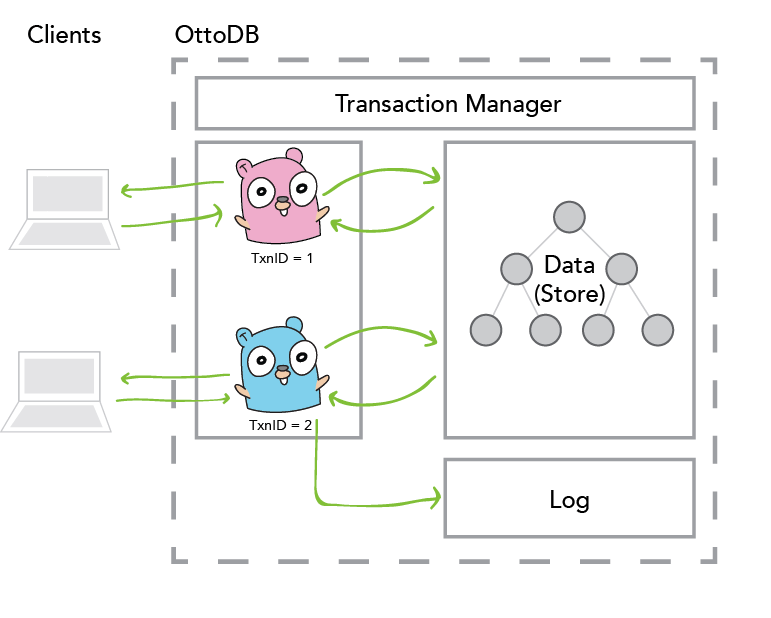
\includegraphics[width=\columnwidth]{figures/OverallArchitecture.png}
    \caption{Overall Architecture}
    \end{figure}

    OttoDB runs as a tcp server, listening to requests to then perform operations on the underlying data storage layer. When a new transaction begins, it's given an atomically increasing transaction id, which is used to determine record visibility. Every client is handled by a separate go routine (lightweight-thread), and interacts directly with an in-memory store of key/value records. Storing data in-memory allows for faster reads/writes on the data as compared to if it was solely stored on disk. As commands come in they are written to an append-only log, which acts as persistent storage. On startup/restart, the log is replayed on the store before any requests are handled. OttoDB's protocol is influenced heavily by that of Redis. OttoDB supports \textit{get}, \textit{set}, and \textit{delete} operations, along with others for transactional control.

    \subsection{Protocol}

    OttoDB supports a similar protocol as Redis \cite{b1}, but with a smaller variability of data stored; OttoDB currently only supports keys and values as strings. The following operations OttoDB supports are shown below.

    \begin{itemize}
        \item BEGIN - Starts a transaction with the client, all future requests are scoped to the transaction.
        \item COMMIT - Lets OttoDB know you're ready to commit the transaction to the store
        \item GET \textit{key} - Returns the string value of the \textit{key}, if it exists. If not, returns an empty string
        \item SET \textit{key} \textit{value} - Sets \textit{value} to \textit{key} in the database or updates previously set key, returns message ‘OK’
        \item DEL \textit{key} - Deletes the record in the database associated with the provided \textit{key}, returns message ‘OK’ on success
        \item ABORT - Rolls back any changes made by the current transaction and ends the transaction
        \item QUIT - Kills the active TCP connection with the database
    \end{itemize}

    Similar to Redis \cite{b1}, all requests are terminated with an {\textbackslash}r{\textbackslash}n string. 

    \subsection{Multi Version Concurrency Control (MVCC)}

    Multi Version Concurrency Control (MVCC), is a technique used in OttoDB for implementing snapshot isolation. Snapshot isolation allows transactions to run as if they are viewing their own version of the database, snapshotted in time. This allows long running read-only transactions to run without interruption from many writing transactions. The main concept of MVCC is that \textit{“readers never block writers, and writers never block readers”} \cite[p. 239]{b18}. 

    \subsection{Serializable Snapshot Isolation (SSI)}

    Although MVCC is a performant isolation level, it's also considered a weak isolation level \cite[p. 261]{b18}. Serializable Snapshot Isolation (SSI) provides full serialization to even weak isolation levels that revolve around the idea of optimistic concurrency control \cite[p. 261]{b18}. It can perform better than true serialized execution and in loads of low contention, better than two-phase commit \cite[p. 265]{b18}. SSI is used by PostreSQL and FoundationDB \cite[p. 261]{b18}. 

    \subsection{Transactional Support}

    The above isolation levels make OttoDB a fully serializable database. In OttoDB, transactions: (1) Are performed all together or not at all. (2) Don't affect other transactions. The second property is handled through an MVCC and SSI implementation. 

    % Storage
    \section{Storage}

    \subsection{LSM-Tree of SSTables for append-only storage}

    The storage layer for OttoDB was inspired by an append-only disk writing approach taken in some databases (LevelDB \cite{b7}, RocksDB \cite{b6}, and Cassandra \cite{b19}). In this approach, data is stored in an in-memory, self-balancing tree. When in-memory storage gets too large, it's flushed into a Sorted String Table (SSTable) \cite[p. 78]{b18}, shown in Figure~\ref{fig:SSTable}. SSTables hold key value pairs, along with a timestamp in sorted order on disk. Paired with keys in sorted order, there's a sparse, in-memory, index map, which holds an offset to a few keys in the table \cite[p. 77]{b18}. 

    %Figure X, SSTable Structure
    \begin{figure}[h]
        \centering
        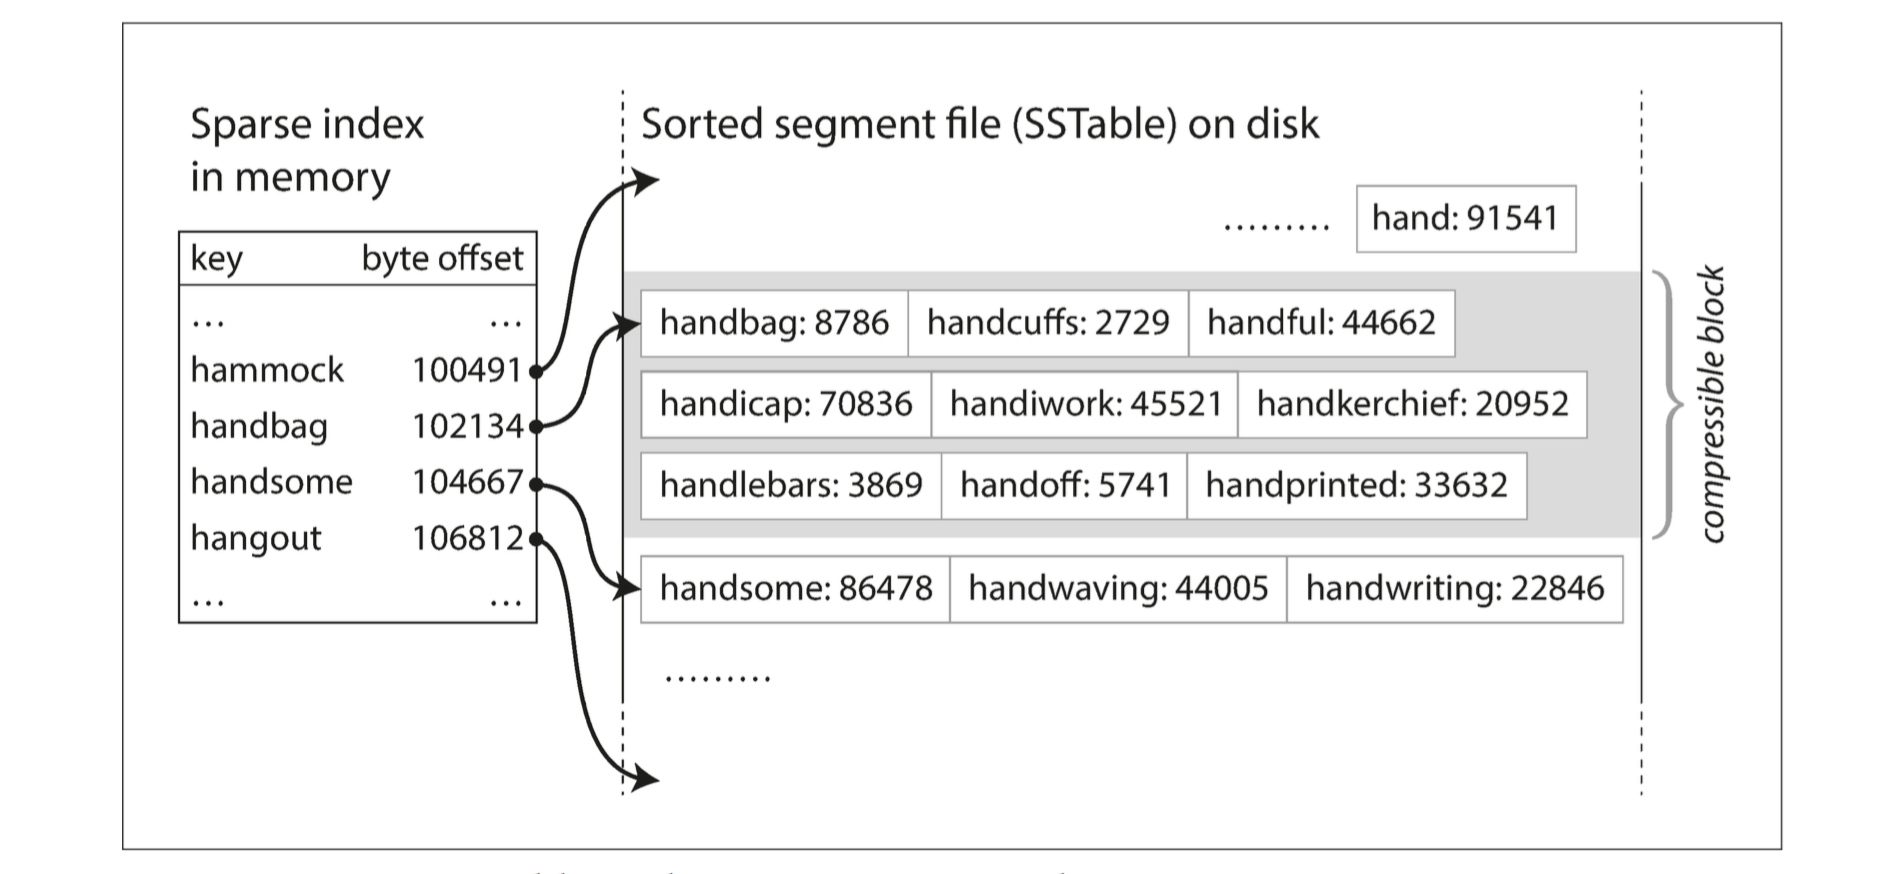
\includegraphics[width=\columnwidth]{figures/SSTable.png}
        \caption{SSTable Structure}
        \label{fig:SSTable}
        \end{figure}

    As the in-memory store keeps getting filled up, it gets flushed to new SSTables. A background process merges tables together with a similar merging algorithm to the merge in merge-sort. Newer timestamps are chosen over older ones, so the data on disk gets compressed. By merging and compacting these appen-only structures, it creates a Log Structured Merge Tree (LSM-Tree). 

    %Figure Y, LSM-Tree compaction 
    \begin{figure}[h]
        \centering
        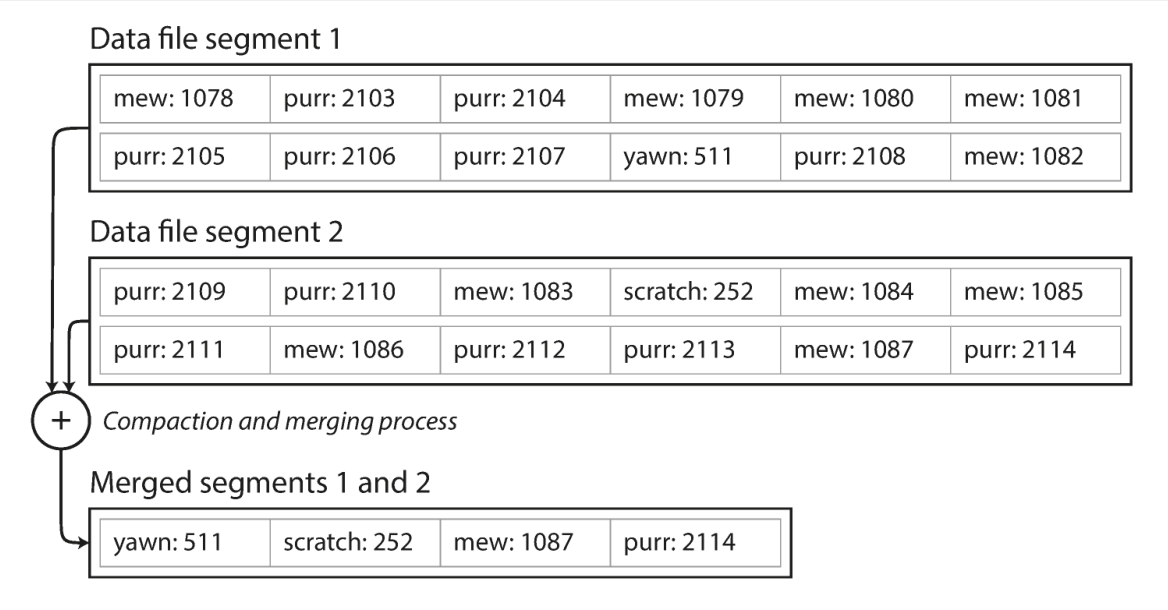
\includegraphics[width=\columnwidth]{figures/LSMTree.png}
        \caption{LSM-Tree Compaction}
        \label{fig:LSMTree}
        \end{figure}

    This data storage approach allows for fast writes to an in-memory structure, but potentially slow read times; you might need to look many SSTables back to find a key \cite[p. 79]{b18}.

    \subsection{OttoDB's in memory storage}

    Originally, OttoDB's in-memory data was stored in a Red Black Tree, to make sure that the tree stayed balanced. Despite the benefits of an always balanced tree, adding concurrency control to the RBTree became difficult. This was because inserting one node could cause any number of tree rotations. This required the entire tree to be locked from other concurrent operations during an insert or delete. Performing a database wide lock on every transaction was not attractive, especially because my goal is to minimize time spent blocking on locks. While researching concurrent RBTree implementations, I found many papers \cite{b20, b21}. These implementations were clever, complex, and couldn't fit in the scope of my project.

    % Figure Wait-free concurrent Red Black Tree Design. Src [\cite{b20}]
    \begin{figure}[h]
        \centering
        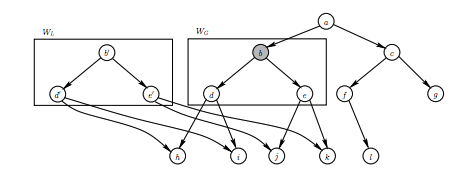
\includegraphics[width=\columnwidth]{figures/ConcurrentRBTree.png}
        \caption{Wait-free Concurrent Red Black Tree Design \cite{b20}}
        \end{figure}

    At the point of implementing concurrency control on the RBTree, I had taken up half of my project development time. I decided to save writing data to SSTables for later, and stick with only an in-memory representation of data, along with a persisted log. Simplifying the storage layer, I changed the RBTree to a  binary tree. This change allowed me to still make the LSM-Tree/SSTable implementation in the future, as well as made concurrent safety much easier to implement.

    % Figure X, Keys stored in tree
    \begin{figure}[h]
        \centering
        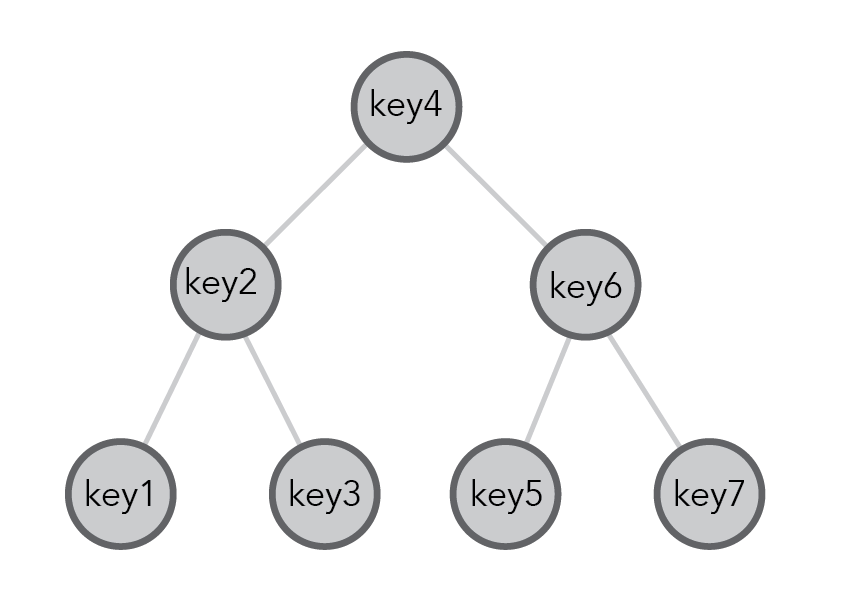
\includegraphics[width=\columnwidth]{figures/binaryTree.png}
        \caption{Keys stored in tree}
        \end{figure}

    \subsection{OttoDB's Write-Ahead Log}

    % Figure Z, Format of log
    \begin{figure}[h]
        \centering
        \includegraphics[width=\columnwidth]{figures/logFormat.png}
        \caption{Protocol Buffer Log Format}
        \end{figure}

    OttoDB utilizes a write-ahead log, as a form of persistence and recovery. In OttoDB, the log is stored as a protocol buffer. Similar to xml and json, protocol buffers are used as a way to serialize data for either storage or message passing \cite{b22}. On startup, OttoDB checks to see if this log exists. If the log exists, all aborted transactions get filtered out, and only previously committed transactions get replayed on a new binary tree. This functionality provides OttoDB with increased durability, as it can handle being shut down while still keeping store state.

    \section{Transaction Isolation}

    Transactions provide a great guarantee to developers. Imagine a database where transactions don't have any isolation. You could write a transaction that reads a value that later on gets aborted. You could also overwrite a value that an active transaction just set, completely losing the update of that transaction. Databases without isolation between transactions can cause utter chaos. 
    
    In order to make developers sane, transactions should be isolated. Just like how we need to protect in-memory data structures with locks or semaphores, transactions need to be protected through isolation. Isolation in transactions is a basic guarantee in almost all databases that help developers with deployed code sleep at night.

    \subsection{Read Committed Isolation}

    Read committed isolation provides the most basic of isolation functionalities. The main functionalities are: (1) A transaction can only read values that have been committed, (2) A transaction can only overwrite values that have been committed. These two guarantees prevent \textit{dirty reads}, and \textit{dirty writes}. \cite[p. 234]{b18}.

    % Figure X, No dirty Reads Src[\cite[p. 234]{b18}] , User 2 only sees the value of 3 until after user 1 has committed.
    \begin{figure}[h]
        \centering
        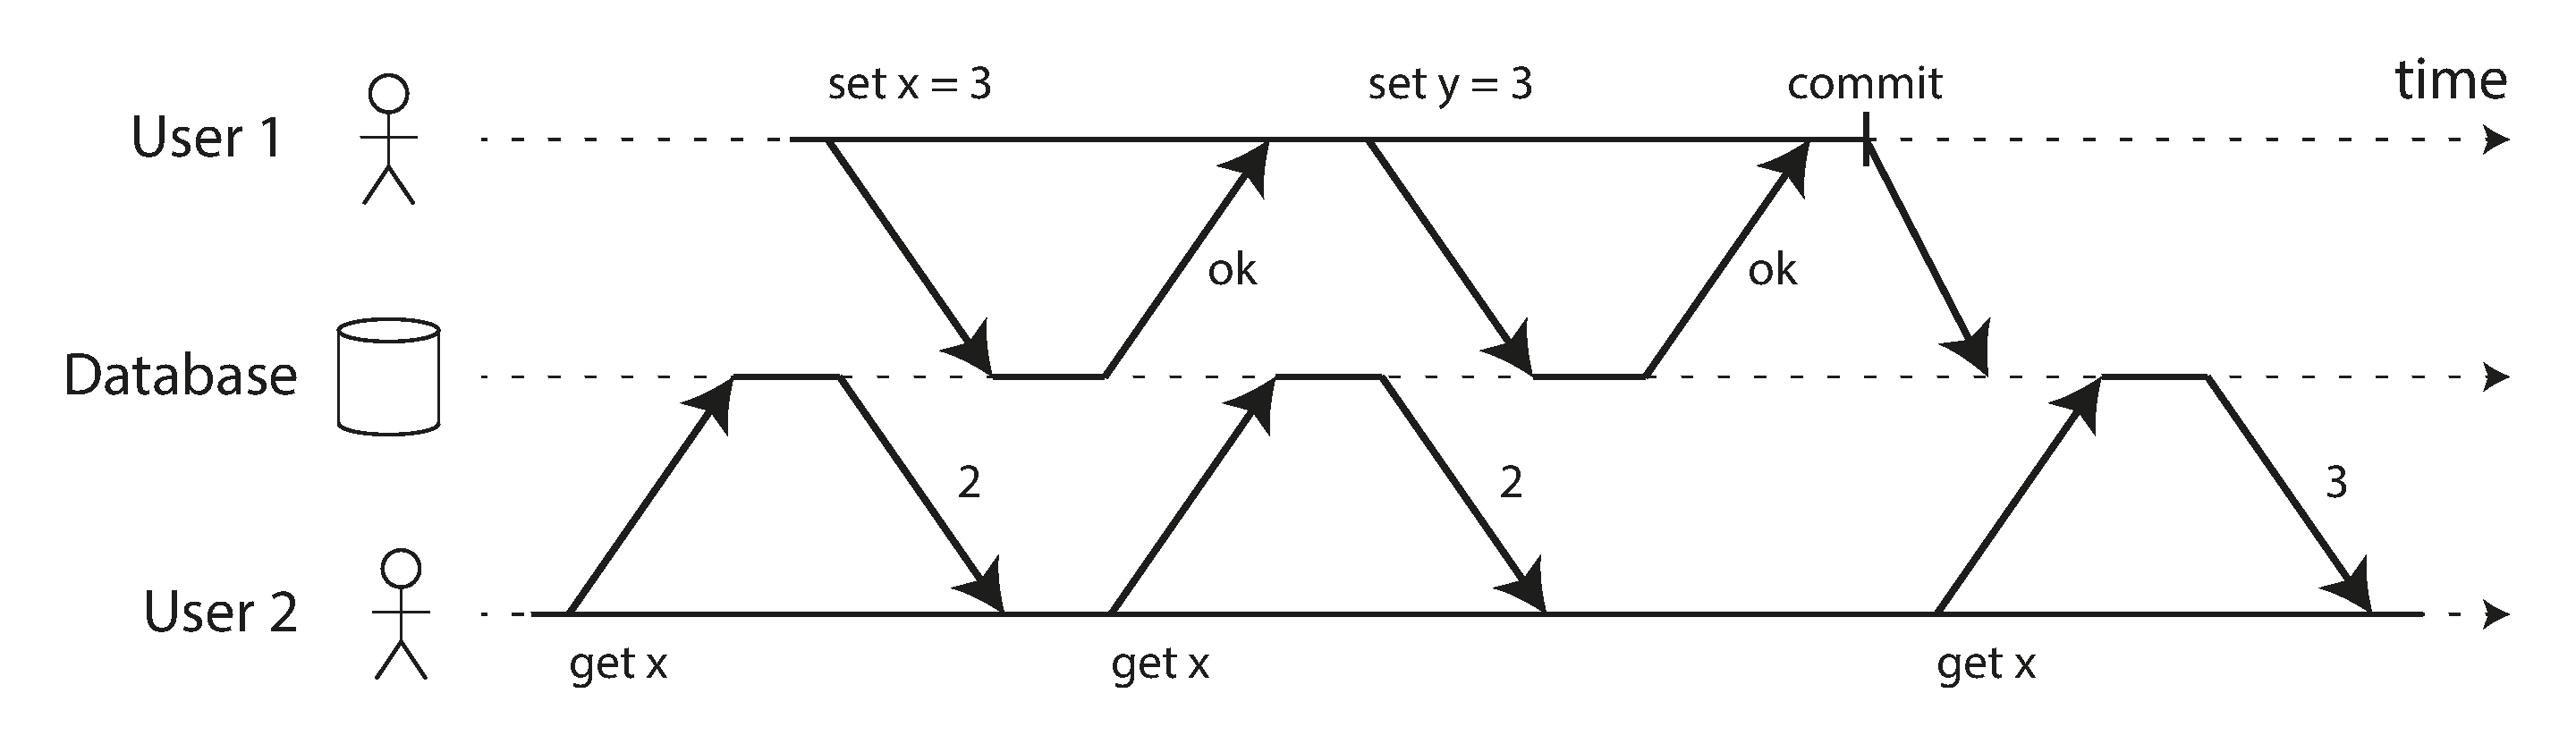
\includegraphics[width=\columnwidth]{figures/NoDirtyRead.png}
        \caption{No Dirty Reads. User 2 only sees the value of 3 until after user 1 has committed \cite[p. 234]{b18}}
        \end{figure}


    % Figure Y, Example of a dirty write. Src [\cite[p. 236]{b18}]
    \begin{figure}[h]
        \centering
        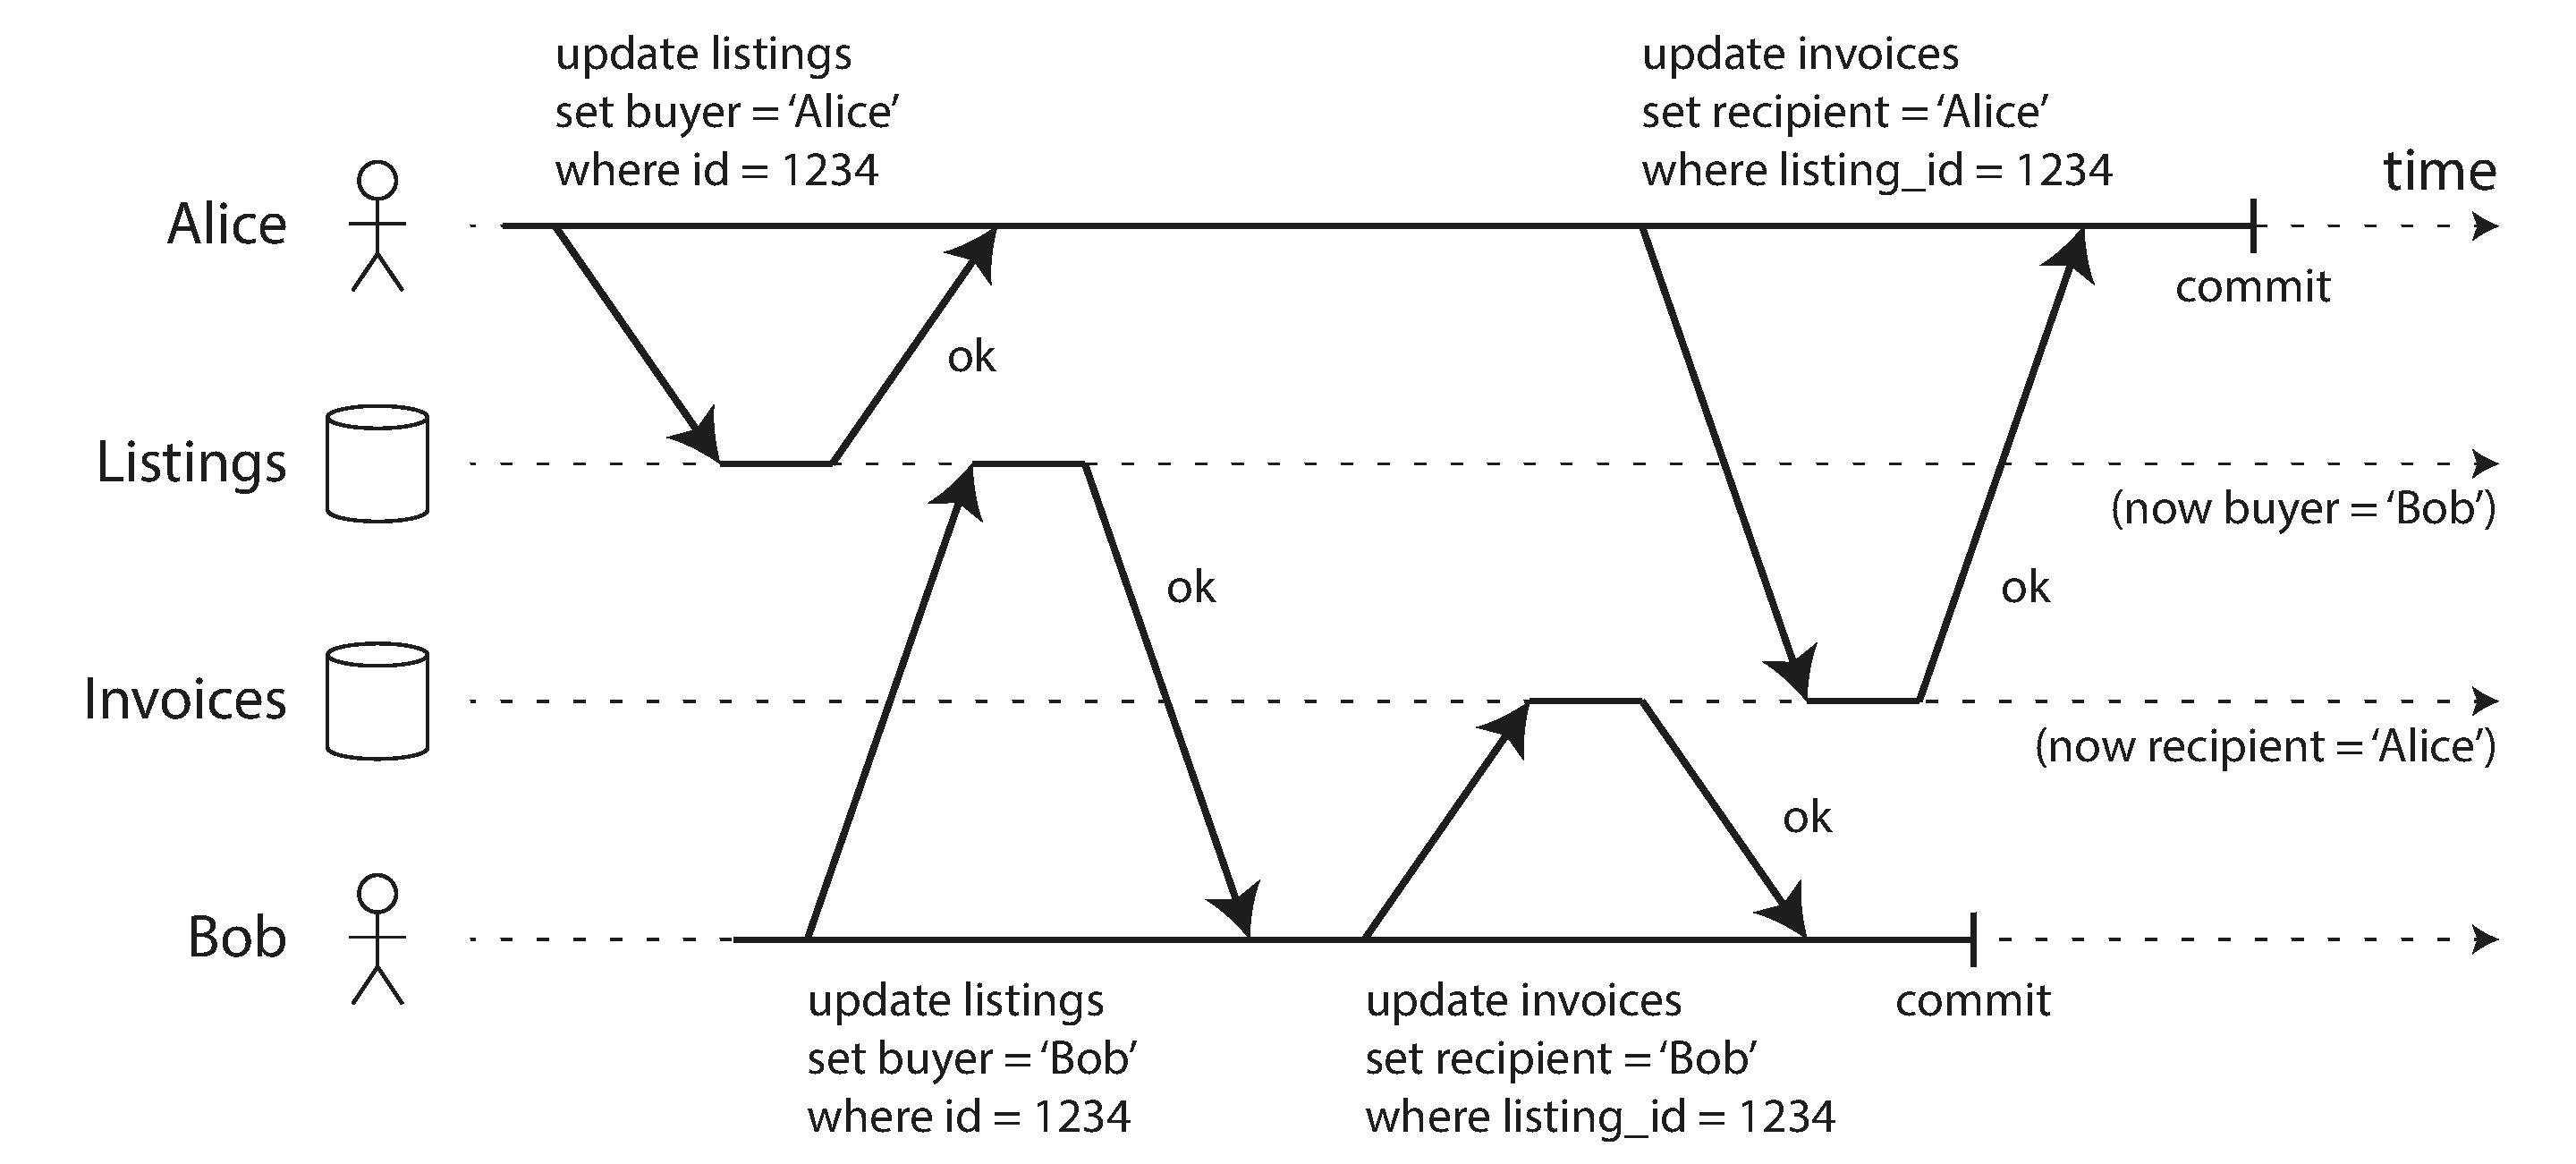
\includegraphics[width=\columnwidth]{figures/DirtyWrite.png}
        \caption{Example of a dirty write \cite[p. 236]{b18}}
        \end{figure}

    Read committed isolation is the default isolation level in PostgreSQL, SQL Server 2012, and MemSQL \cite[p. 236]{b18}. This technique is simple, but has some major performance drawbacks. The main issue with read committed isolation is that transactions hold onto locks of the values the read or write until their transaction commits or aborts \cite[p. 236]{b18}. If a long write-heavy transaction is running, it can prevent smaller read-only transactions from making progress, as they will block until the write-heavy transaction's locks are freed.

    % Figure Z, Example of read skew Src[\cite[p. 237]{b18}]
    \begin{figure}[h]
        \centering
        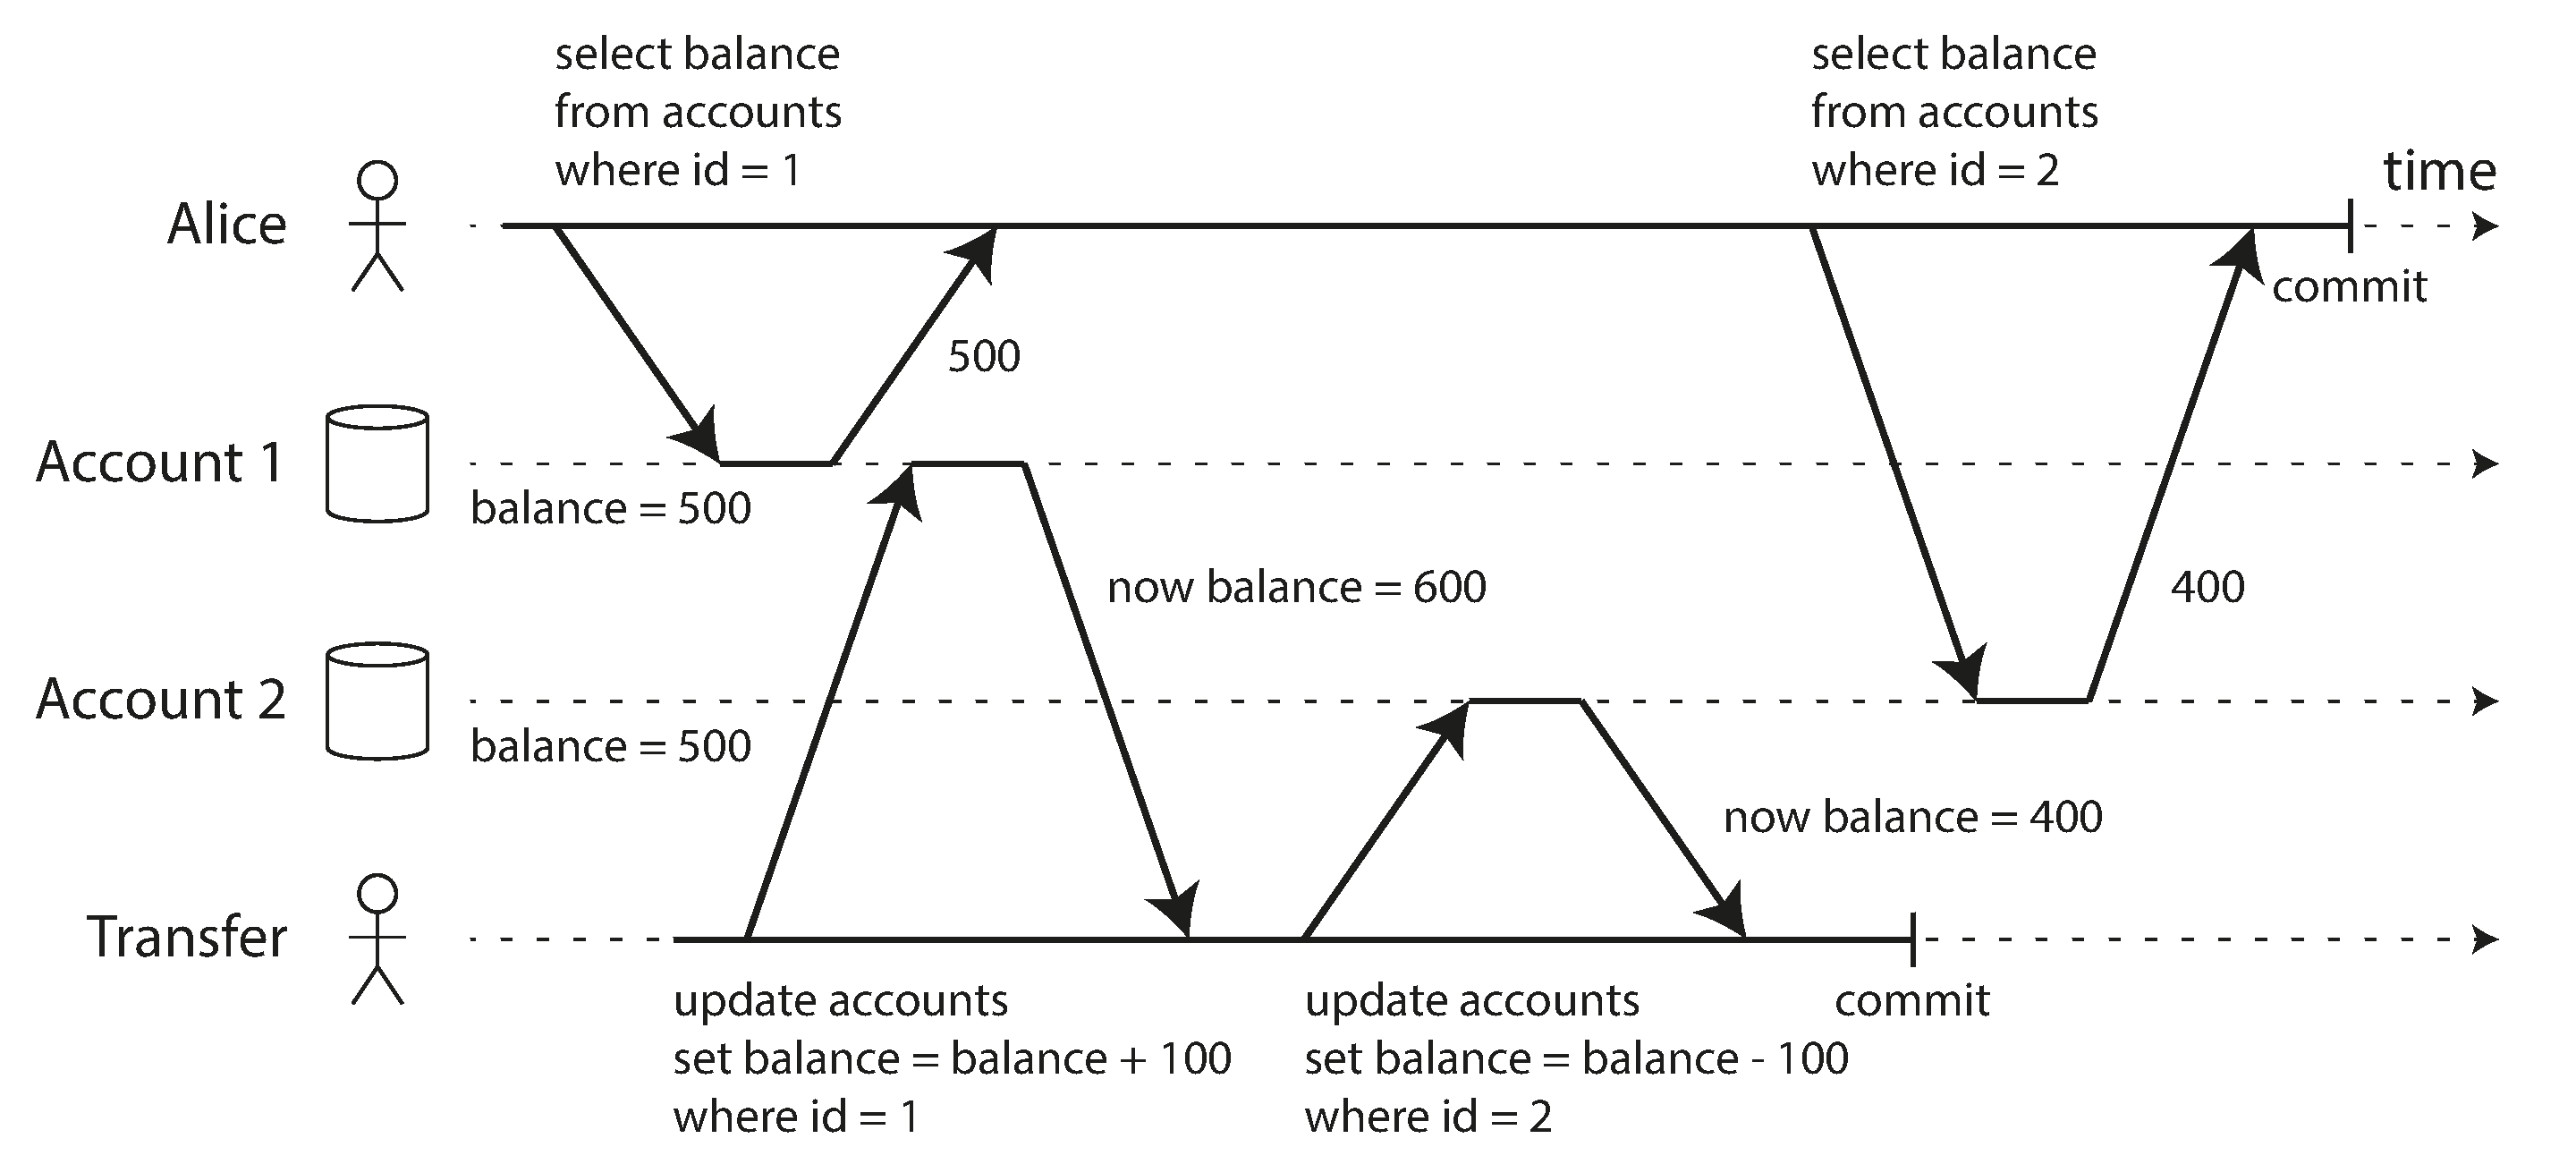
\includegraphics[width=\columnwidth]{figures/ReadSkew.png}
        \caption{Example of read skew \cite[p. 237]{b18}}
        \end{figure}

    Another downfall of read committed isolation is that it's susceptible to \textit{read skew} \cite[p. 237]{b18}. If a transaction were to read a value once, that value gets overwritten by a committing transaction, if the transaction reads that value again it will get a different result. Read skew can affect a database when it's being backed up, by providing it an inconsistent view of the database \cite[p. 237]{b18}. It can also be tough for analytic queries, as they could return an inconsistent view of the data \cite[p. 237]{b18}. I wanted OttoDB to be as transactionally safe as possible, so a read committed isolation level was not a valid isolation target.

    \subsection{Snapshot Isolation}

    Snapshot isolation provides the same protections that read committed does, and also protects from \textit{read skew}. The main idea behind snapshot isolation is that a transaction “sees all the data that was committed in the database at the start of the transaction. Even if the data is subsequently changed by another transaction, each transaction sees only the old data from that particular point in time” \cite[p. 238]{b18}. This isolation level is supported in many of the most popular databases \cite[p. 239]{b18}. 
    
    In order to provide this functionality to long running queries, multiple versions of each record are stored. This allows older transactions to read versions of data in their own snapshot while newer transactions can read data that has been committed before them.

    \subsection{OttoDB's Snapshot Isolation Implementation}

    % ** Figure showing the unique transaction number and idea behind the snapshot (only older committed txn values are present) **

    OttoDB stores multiple versions of a key through a technique called Multi Version Concurrency Control (MVCC). When a transaction is started, its first given a unique transaction-id. This transaction-id is used to determine which versions of data a transaction can view or overwrite. Transactions in MVCC can only view data from committed transactions that came before the transaction began.

    % Figure Y, Multiple versions of a record
    \begin{figure}[h]
    \centering
    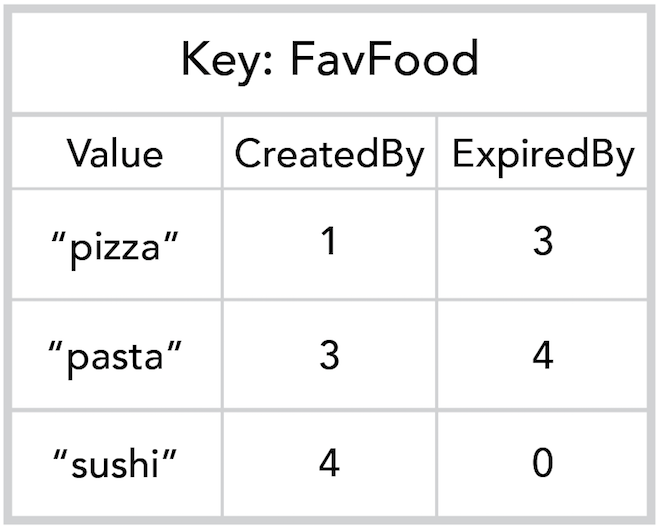
\includegraphics[width=\columnwidth]{figures/MVCCDetail.png}
    \caption{Overall Architecture}
    \end{figure}

    In OttoDB's implementation of MVCC, keys are stored as lists of records, which contain all versions of a key. Along with the key's value, records have two additional propertires: \textit{CreatedBy}, and \textit{ExpiredBy}. The \textit{CreatedBy} field holds the transaction id of the transaction that wrote it. The \textit{ExpiredBy} field holds the transaction id of the transaction that deleted it. 
    
    When a transaction reads a value, it starts at the most recent version, and works its way backward in time until it finds a version it has visibility to read. Visibility on a record is not met if any of the following conditions are true:

    \begin{itemize}
        \item CurrentRecord.Status = Aborted
        \item CurrentRecord.CreatedBy \textgreater \space txnId
        \item CurrentRecord.CreatedBy is an active txn AND CurrentRecord.CreatedBy != txnId 
    \end{itemize}

    % Figure of delete

    When a delete is performed, it doesn't remove the record from memory, as that could affect earlier transactions that need to read the value. Instead of removing the value, delete operations mark the record for deletion, by setting the \textit{ExpiredBy} value to their own transaction id \cite[p. 240]{b18}. If the transaction is committed, future transactions will not be able to view that record, as their transaction-id is greater than the record's \textit{ExpiredBy} value. 

    % Figure Y, Example insert operation Src \cite[p. 240]{b18}
    \begin{figure}[h]
        \centering
        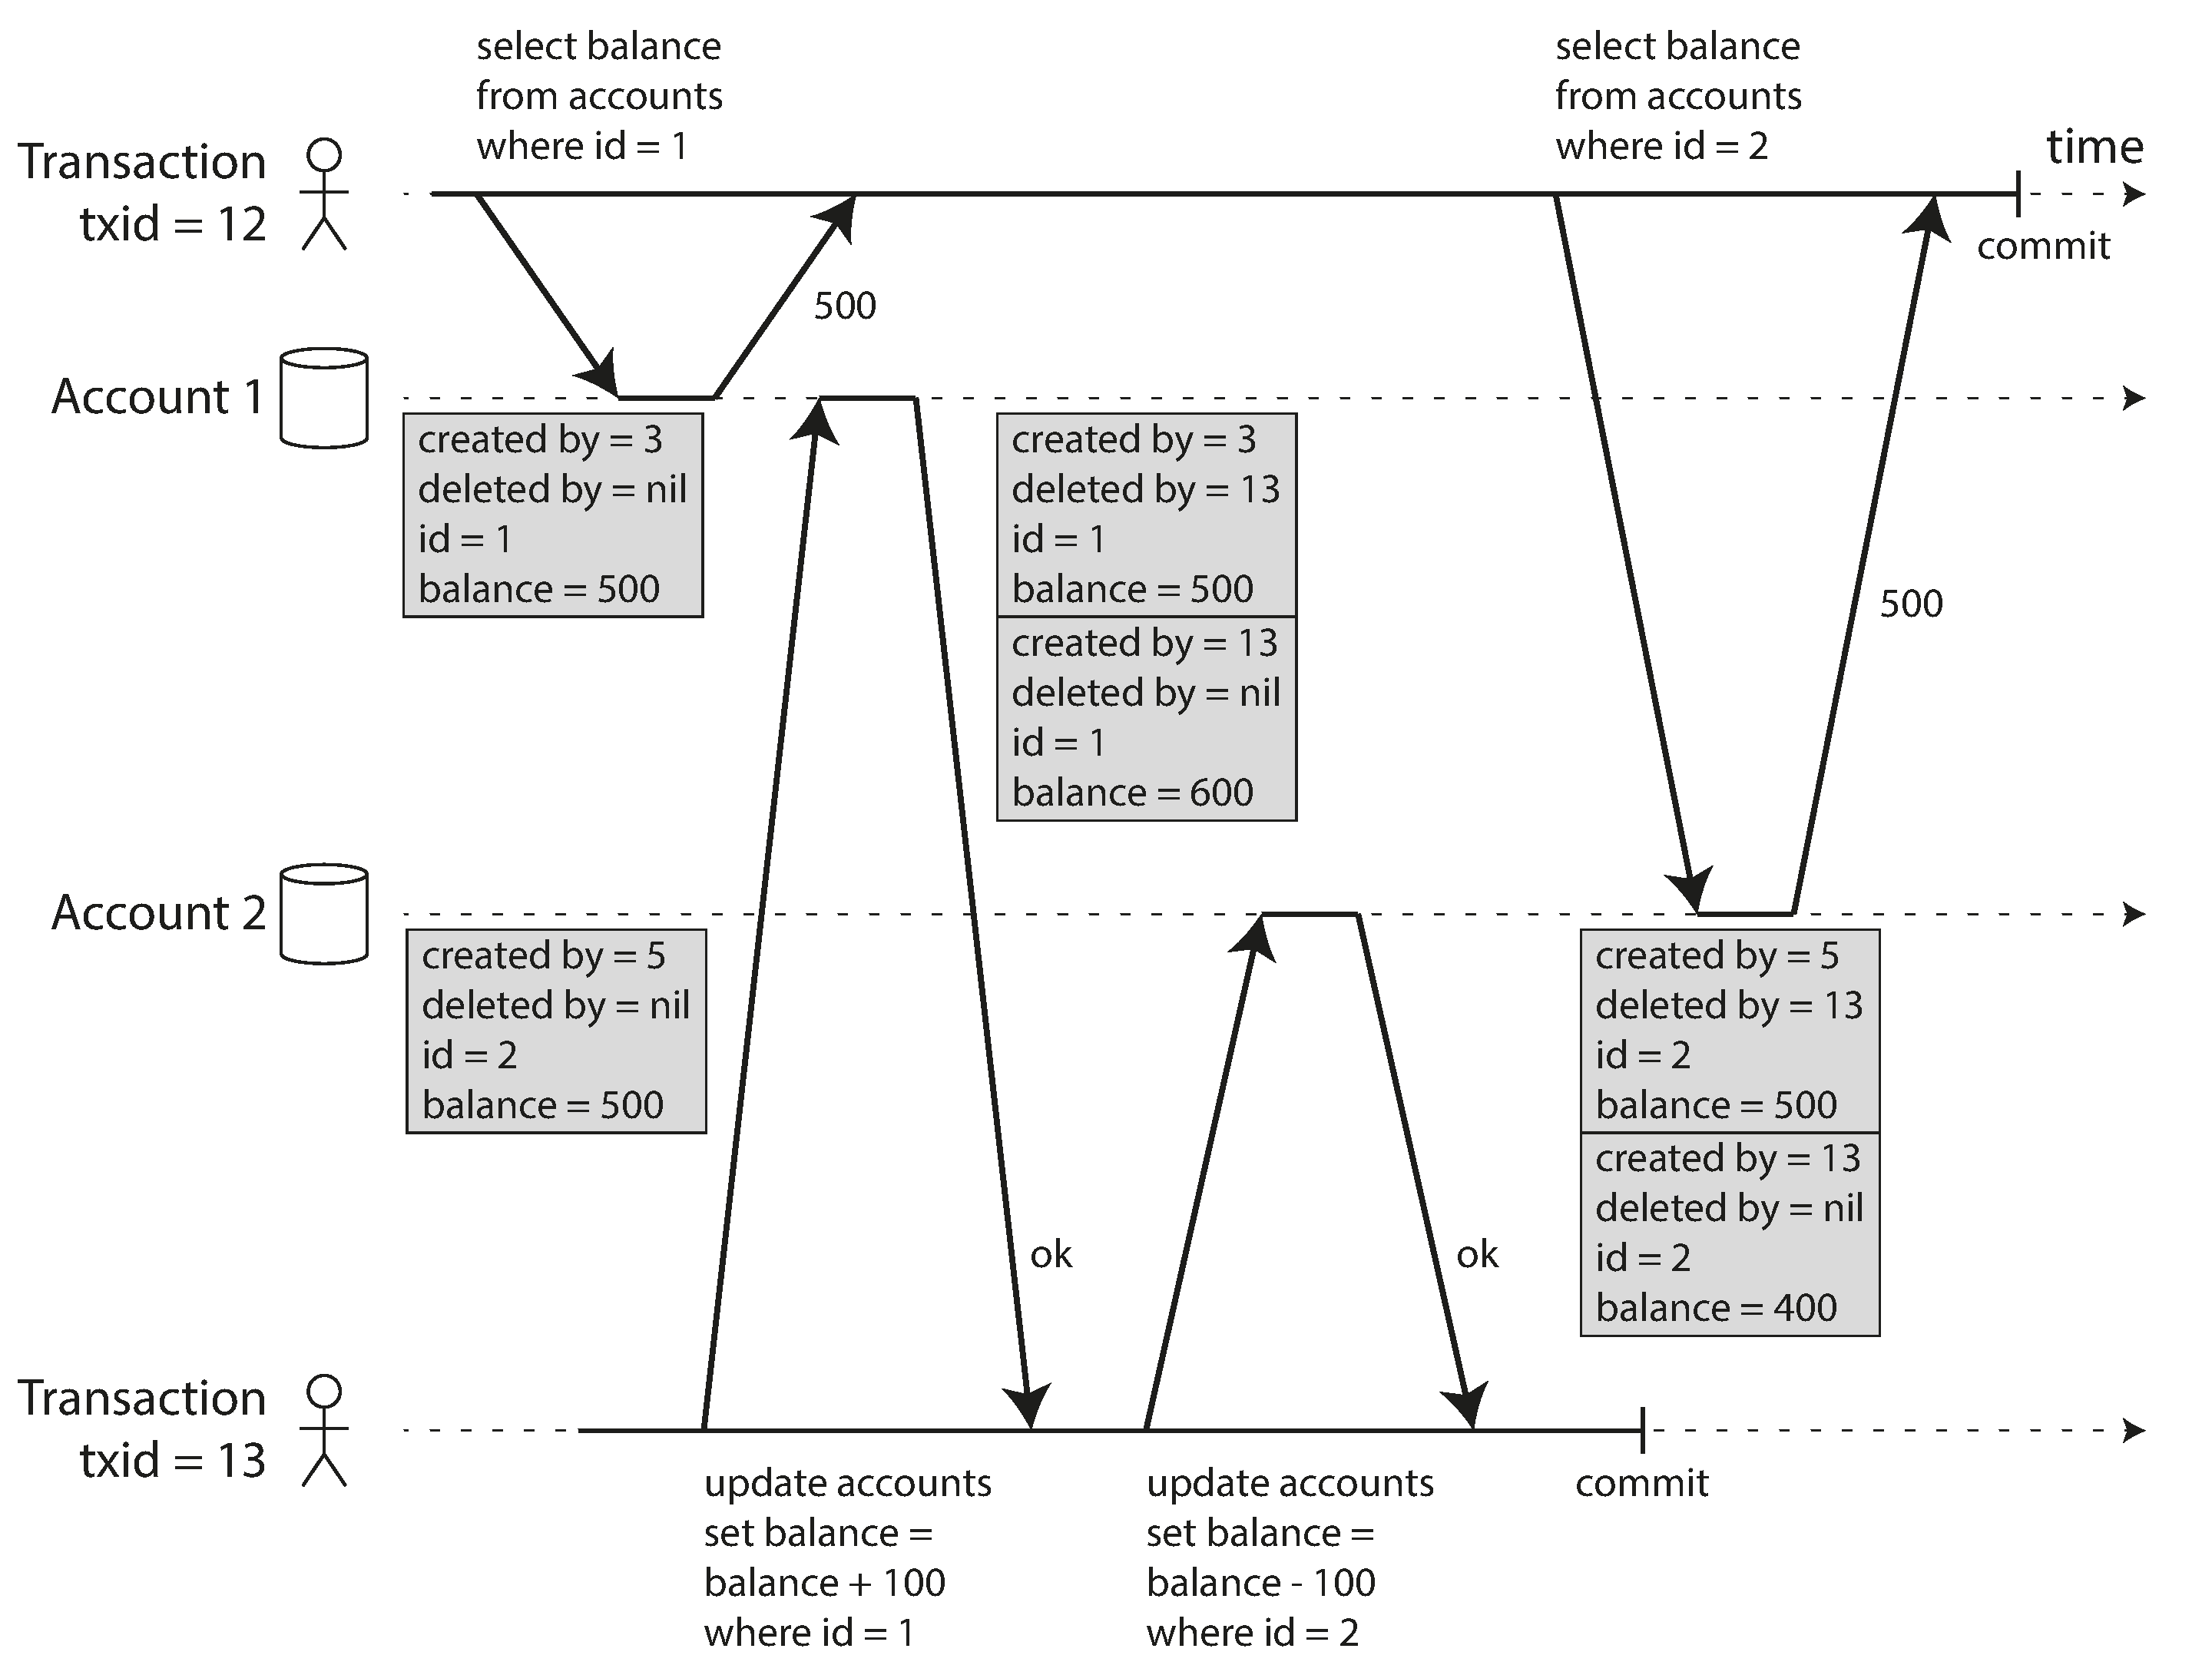
\includegraphics[width=\columnwidth]{figures/MVCCInAction.png}
        \caption{Example insert operation \cite[p. 240]{b18}}
        \end{figure}

    Inserts are performed by first marking the current version of a record for deletion \cite[p. 240]{b18}. After expiring the current version, a new record is appended to the version list with it's \textit{CreatedBy} id as the current transaction id and an \textit{ExpiredBy} value of 0. 
    
    MVCC snapshot isolation protects OttoDB from dirty reads, dirty writes, and read skew, but there aren't rules about overwriting records, which leaves it open to the lost update problem. 
    
    % Figure of the transactions that create a lost update problem **
    
    The lost update problem occurs when multiple transactions read from a value, modify that value, and then write that value back to the database \cite[p. 243]{b18}. This situation can have one transaction's write clobber the other, because it didn't see the previous transactions updated value when reading \cite[p. 243]{b18}. There are many solutions to this problem: Atomic Write Operations, Explicit Locking, Automatically Detecting Lost Updates, and Compare-and-Set operations \cite[p. 243 - 245]{b18}. OttoDB uses a set of rules on deletes and writes, similar to that of reads, to protect transactions from the lost update problem.
    
    A transaction in OttoDB can not write or delete on a record list if any of the following is true:

    \begin{itemize}
        \item record.CreatedBy \textgreater \space txnID
        \item record.CreatedBy is an active transaction AND is not the current txnID
        \item record.ExpiredBy \textgreater \space txnID
        \item record.ExpiredBy is an active transaction AND is not the current txnID
    \end{itemize}
 
    In OttoDB, a key's version list is held in a \textit{go slice}, which is a sorted, dynamic collection of elements. Although in a pure MVCC approach, there would only be write locks and no read locks, I have each key's record list protected by a Read/Write Mutex lock. This means that OttoDB doesn't receive the full performance benefits of MVCC. It does however, receive the isolation benefits of keeping \textit{dirty reads}, \textit{dirty writes}, \textit{read skew} and \textit{lost updates} from occurring.

    \section{Serlializable Transactional Isolation}

    For transactions to be fully isolated, they need to meet the second property we've set for transactions: (2) A transaction shouldn't affect other concurrent transactions. Through OttoDB's MVCC isolation level, only a subset of concurrent errors are avoided. Although MVCC protects from \textit{dirty writes}, it mostly takes care of errors with reading values. With only MVCC, the database is still susceptible to \textit{write skew} \cite[p. 246]{b18}.

    % Figure Y, Write Skew Src[\cite[p. 247]{b18}]
    \begin{figure}[h]
        \centering
        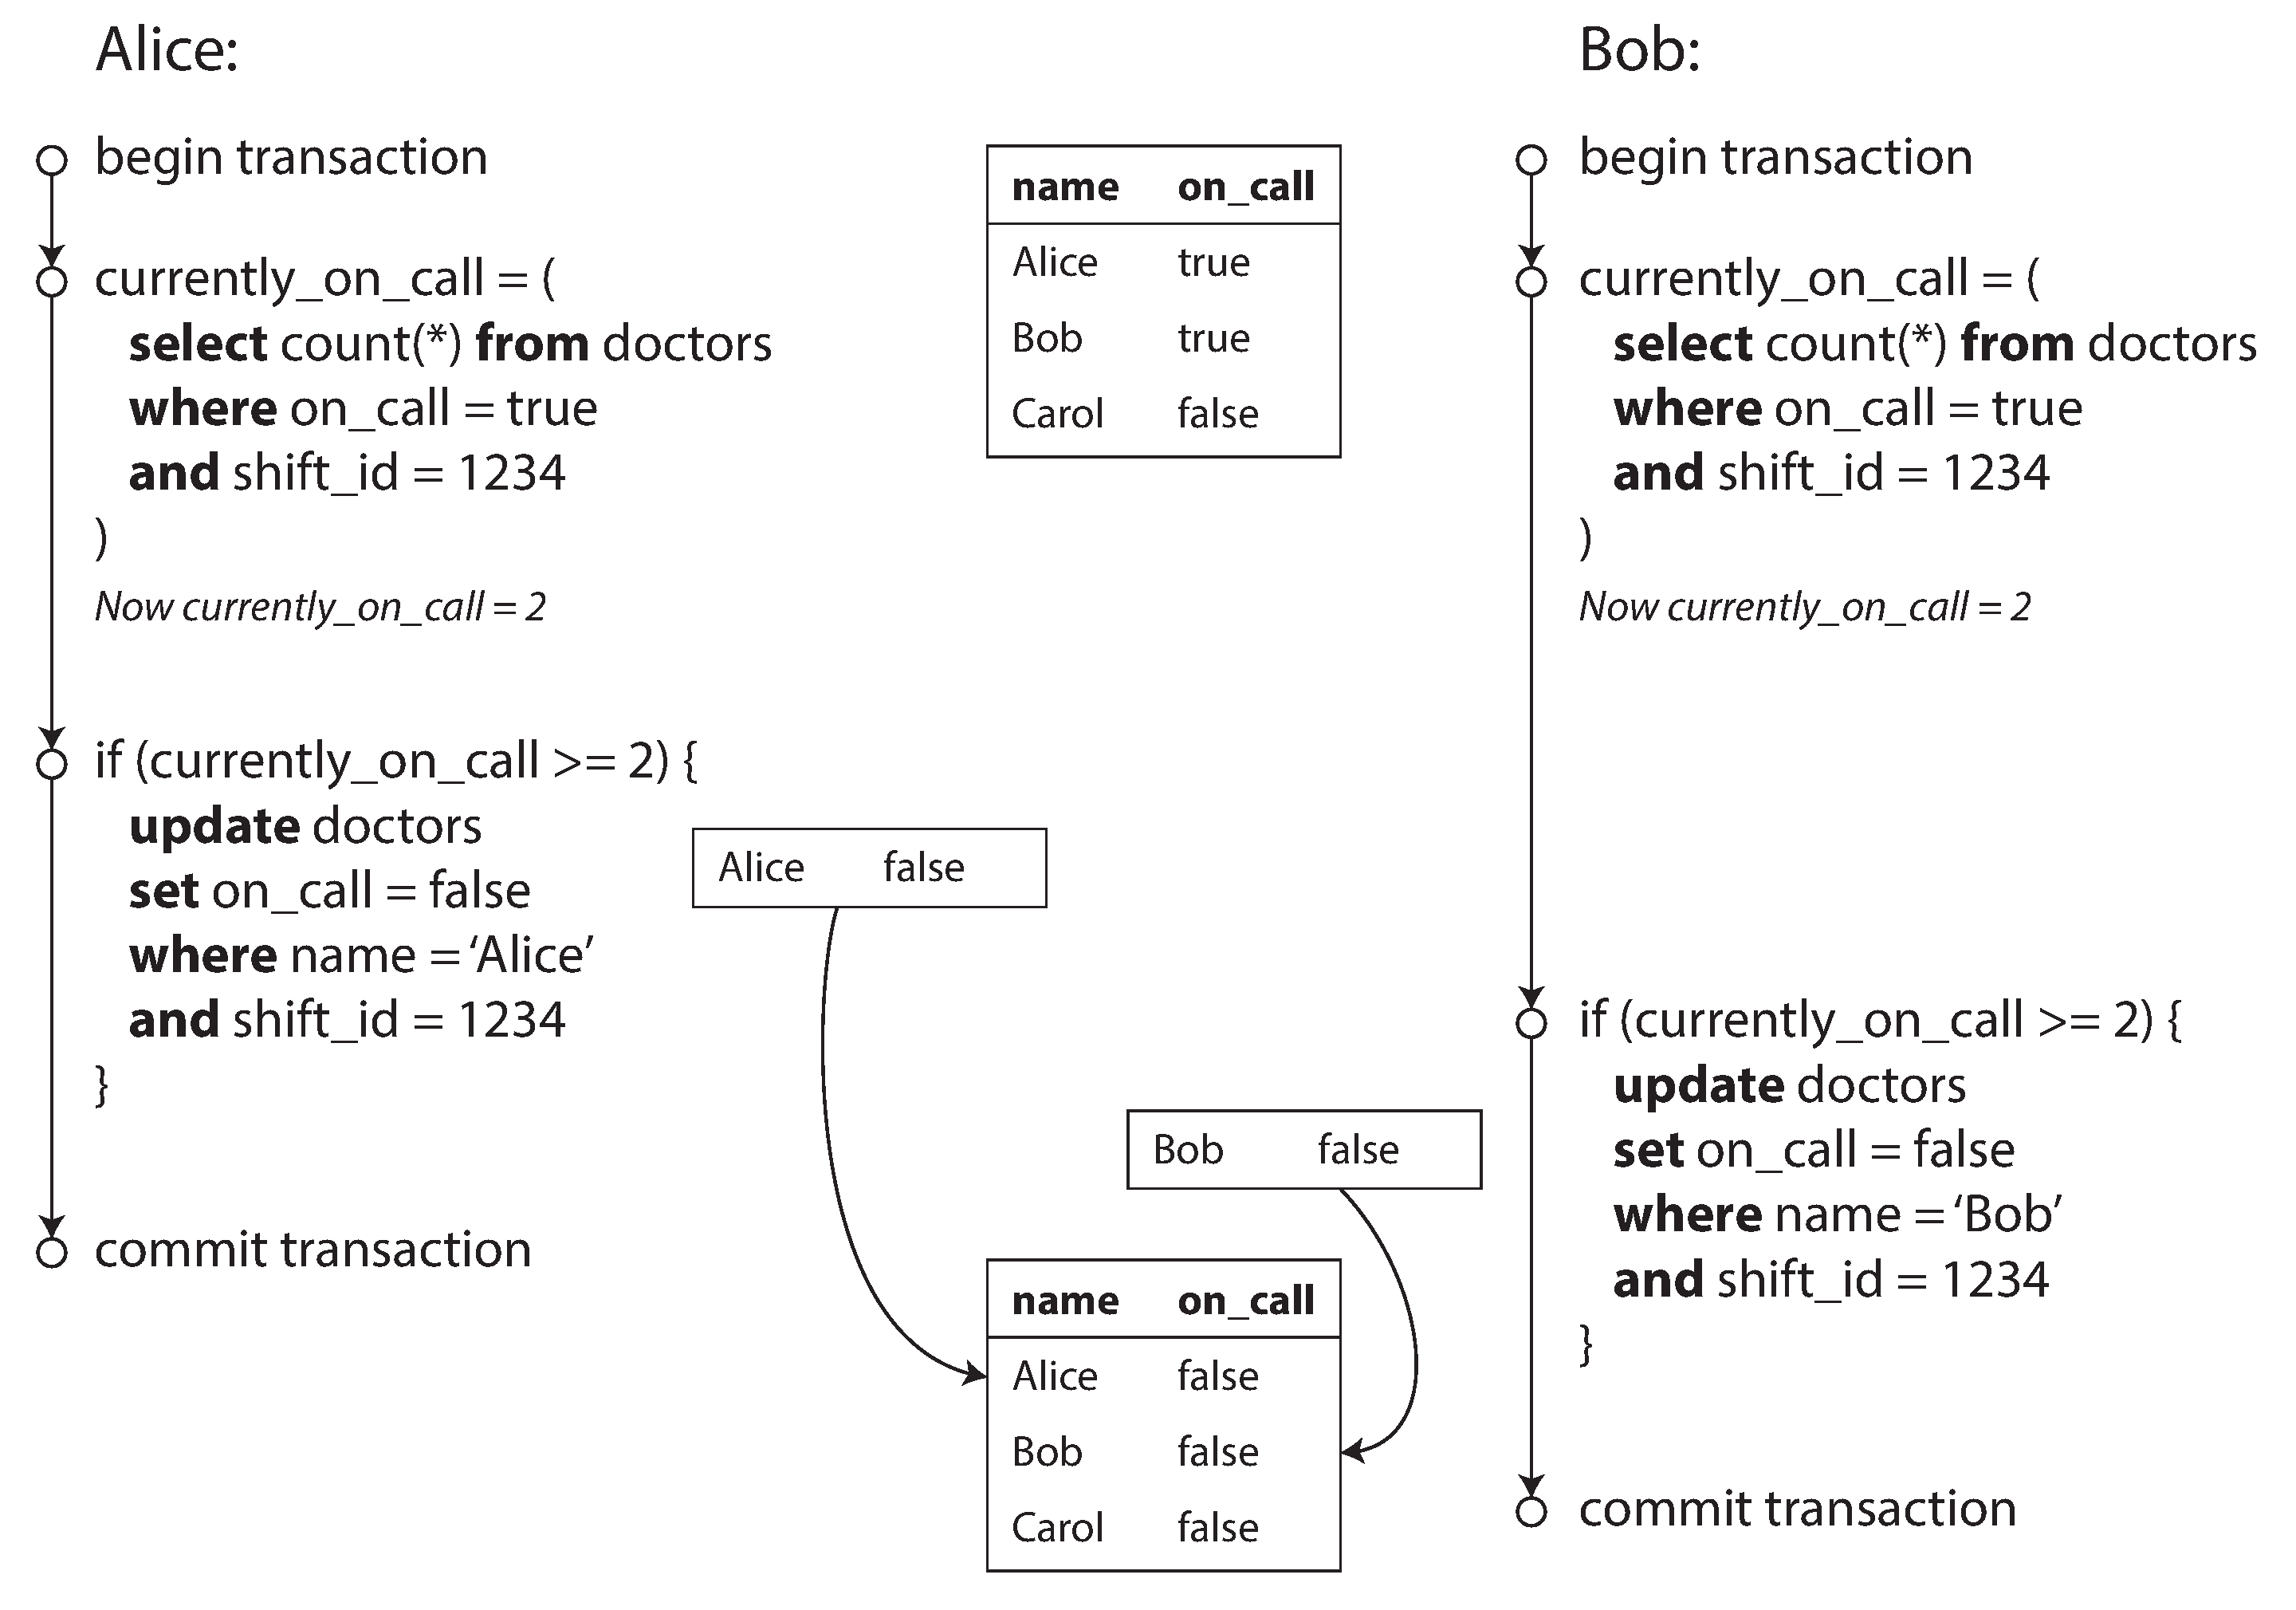
\includegraphics[width=\columnwidth]{figures/WriteSkew.png}
        \caption{Write Skew \cite[p. 247]{b18}}
        \label{fig:WriteSkew}
        \end{figure}

    A popular example of write skew is that of two doctors who are sick, and need to take time off. At the hospital, there should be at least one doctor available to work. Both Alice and Bob are sick and want to take the day off. They both start a request to the database that checks if there are 2 or more doctors on call, and if there is, they get taken off call. In the execution order in Figure~\ref{fig:WriteSkew}, both of their transactions are working on the premise that the other doctor hasn't asked for time off. This leads to no doctor's working at the hospital and leaves the application in an erroneous state. 
    
    Even though the issue comes from updating two separate records, it's still considered a race condition \cite[p. 247]{b18}. This issue isn't solved by the lost update or dirty reads/writes solutions. Write skew is a generalization of the lost update problem mentioned earlier; two transactions read the same objects, and then update some of those objects \cite[p. 248]{b18}. To solve this, a different isolation level needs to be added to OttoDB, serializable isolation. There are multiple solutions to implementing serializable isolation, which I will introduce to later compare to the strategy taken in OttoDB.

    \subsection{Actual Serial Execution}

    Actual serial execution takes the opinion of, \textit{Why try to manage all these threads to provide serializable isolation? Just use one!} Actual serial execution performs each transaction in actual serial order \cite[p. 253]{b18}. To help improve performance, transactions are usually kept small, and compacted into stored procedures \cite[p. 253]{b18}. Actual serial execution is used in Redis for serializable isolation \cite[p. 253]{b18}. I find this really impressive, because Redis is one of the most performant key value stores, and it runs transactions on a single thread. Actual serial execution benefits from simplicity (not having to manage multiple threads), but could grow slow (i.e. a long running transaction blocking smaller transactions that want to run.

    \subsection{Two Phase Locking (2PL)}

    Two Phase Locking (2PL) is a way to provide serializable isolation for multi-threaded environments. In 2PL, readers wait for locks on objects they want to read, and writers hold exclusive locks on what they want to write \cite[p. 257]{b18}, until their transaction has completed. Two phase locking is considered to be a pessimistic concurrency strategy, as \textit{“writers block readers, and readers block writers”} \cite[p. 257]{b18}. 2PL is used as the serializable isolation level for MySQL and SQL Server \cite[p. 257]{b18}. 2PL suffers from slower response times and transaction throughput when compared to weaker isolation levels (e.g. snapshot isolation) \cite[p. 258]{b18}.

    \subsection{Serializable Snapshot Isolation}

    Serializable Snapshot Isolation (SSI), similar to 2PL, provides serializability to transactions running in a multi-threaded environment. SSI is able to provide full serializability, but at a smaller cost than 2PL \cite[p. 261]{b18}. SSI is an optimistic concurrency control strategy. That means, instead of blocking when something bad could happen (e.g. write skew), SSI waits to see if anything bad does happen, and aborts a conflicting transaction if it does \cite[p. 261]{b18}. There are multiple implementation options for SSI, but they all revolve around detecting when a transaction has made a stale read and updates a value, or when a transaction makes a read-modify cycle on a value that gets changed before it commits.

    \subsection{OttoDB's Serializable Snapshot Isolation Implementation}

    Currently in the works! I'll be able to add this section once completed! I have the design, just need to make it work!

    \section{Related Work}

    OttoDB is a Frankenstein of optimistic concurrency control, married with the limitations of project scope and my lack of experience in database design. Although it utilizes optimistic concurrency control through both MVCC and SSI, it's not the first to do so.
    
    PostgreSQL was born from the idea of optimistic concurrency control \cite{b25} and has had an SSI option of serialization isolation since version 9.1 \cite[p. 261]{b18}. A paper from PostgreSQL \cite{b25}, was the main inspiration for the SSI implementation in OttoDB.
    
    Cockroach DB \cite{b8}, a distributed sql database written in Go, also utilizes MVCC to improve performance of their distributed database. Along with their documentation \cite{b9,b10}, many talks they've done provided insight on how MVCC works \cite{b23, b24}. There is also a key value store written in Go called MOSS (Memory Oriented Sorted Segments). A talk by one of its engineers, Marty Schoch, provided me with insight on how to implement a key value store in Go \cite{b26}. Redis, of course, was a huge influence on the protocol for OttoDB. 
    
    The entire design of OttoDB was heavily influenced by the discussions, and topics covered in Martin Kleppmann's book \cite{b18}. The optimistic concurrency control explanations from his book provided  implementation details for the MVCC system, the in-memory storage implementation, a high-level SSI design, as well as the write-ahead log. I would highly suggest it to anyone interested in distributed applications.

    \section{Experimental Set Up}

    \subsection{Load / Stress Tests}

    One advantage of using a Redis based protocol, is that I can take utilize the redis benchmarking tool for testing. All benchmarking tests are performed on my 2011 Macbook Pro.

    % Figure Computer details
    \begin{figure}[h]
        \centering
        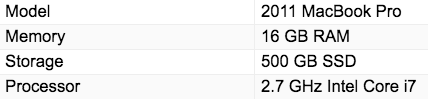
\includegraphics[width=\columnwidth]{figures/ComputerInfo.png}
        \caption{Testing Computer Details}
        \end{figure}

    I will perform load tests, by slamming both Redis and OttoDB with thousands of requests. The two main variables of these tests will be the number of concurrent clients, and the amount of requests. I will be testing a range of 50 to 100 concurrent clients and 5,000 to 100,000 requests.

    \subsection{Serializability Tests}

    Along with load testing the system, I will be performing manual tests to prove that OttoDB provides full serializability and safety from the following conditions: \textit{dirty writes}, \textit{dirty reads}, \textit{read skew}, and \textit{write skew}. Below are labeled transaction executions that are the tests I'll be using to prove OttoDB's full serializability.

    **Tests coming soon!

    \section{Results}

    % Make these bold instead
    \subsubsection{5,000 Requests, 50 Concurrent Clients}
    
    Early Results
    % Figure of early results
    \begin{figure}[h]
        \centering
        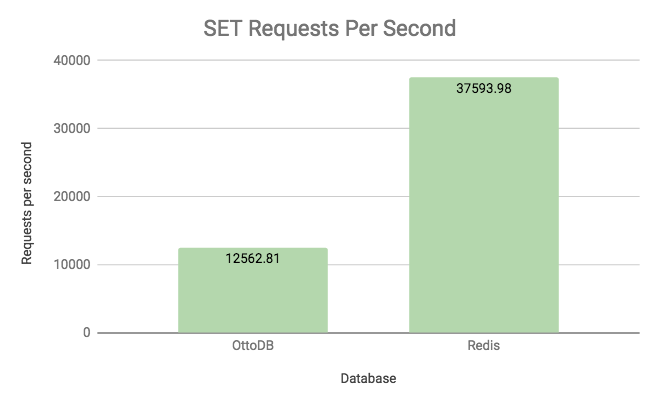
\includegraphics[width=\columnwidth]{figures/5000SetRequests.png}
        \caption{5,000 Requests, 50 Concurrent Clients}
        \end{figure}

    \subsubsection{100,000 Requests, 50 Concurrent Clients}

    *Results coming soon

    \subsubsection{100,000 Requests, 100 Concurrent Clients}

    *Results coming soon

    \subsubsection{100,000 Requests, 100 Concurrent Clients}

    *Results coming soon

    \subsubsection{Dirty Reads}

    \subsubsection{Dirty Writes}

    \subsubsection{Read Skew}

    *Results coming soon

    \subsubsection{Lost Update}

    *Results coming soon

    \subsubsection{Write Skew}

    *Results coming soon


    \section{Summary, Conclusion, Future Work}

    Although OttoDB doesn't stand up against the performance of Redis, it does provide transactional capabilities that Redis does not. Redis's performance is very impressive, especially considering that I was testing against a single-threaded instance of Redis, and it's more common to spin up multiple Redis instances. This project has showed me that throwing more threads at a problem, might not necessarily be faster, it all comes down to the implementation, and what you're willing to give up for more speed. 
    
    I'm proud of what I was able to create through this project. I came in not knowing anything about database internals, and I'm leaving with a much deeper understanding of the trade-offs database designers make. There were many parts of the project I wish to of explored more. For example, when trying to improve the concurrency of my original red black tree implementation, I got introduced to copy-on-write data structures. This led me to start researching Software Transactional Memory (STM). STM is a fascinating approach to handling concurrent operations on data structures and I wish I had more time to try and experiment with something similar.
    
    I plan on adding a more involved persistence layer in the future by implementing the full SSTable LSM-Tree design. I also plan on improving the performance of OttoDB, as it hasn't been refined much after meeting requirements. It would also be interesting to try and distribute OttoDB across multiple machines by using various distributed consensus algorithms we've discussed in class (e.g. Raft, Paxos...etc), but that would come much later.


    % \begin{algorithm}
    %     \KwData{this text}
    %     \KwResult{how to write algorithm with \LaTeX2e }
    %     initialization\;
    %     \While{not at end of this document}{
    %      read current\;
    %      \eIf{understand}{
    %       go to next section\;
    %       current section becomes this one\;
    %       }{
    %       go back to the beginning of current section\;
    %      }
    %     }
    %     \caption{How to write algorithms}
    % \end{algorithm}

    % \subsection{Maintaining the Integrity of the Specifications}
    
    % The IEEEtran class file is used to format your paper and style the text. All margins, 
    % column widths, line spaces, and text fonts are prescribed; please do not 
    % alter them. You may note peculiarities. For example, the head margin
    % measures proportionately more than is customary. This measurement 
    % and others are deliberate, using specifications that anticipate your paper 
    % as one part of the entire proceedings, and not as an independent document. 
    % Please do not revise any of the current designations.
    
    % \section{Prepare Your Paper Before Styling}
    % Before you begin to format your paper, first write and save the content as a 
    % separate text file. Complete all content and organizational editing before 
    % formatting. Please note sections \ref{AA}--\ref{SCM} below for more information on 
    % proofreading, spelling and grammar.
    
    % Keep your text and graphic files separate until after the text has been 
    % formatted and styled. Do not number text heads---{\LaTeX} will do that 
    % for you.
    
    % \subsection{Abbreviations and Acronyms}\label{AA}
    % Define abbreviations and acronyms the first time they are used in the text, 
    % even after they have been defined in the abstract. Abbreviations such as 
    % IEEE, SI, MKS, CGS, ac, dc, and rms do not have to be defined. Do not use 
    % abbreviations in the title or heads unless they are unavoidable.
    
    % \subsection{Units}
    % \begin{itemize}
    % \item Use either SI (MKS) or CGS as primary units. (SI units are encouraged.) English units may be used as secondary units (in parentheses). An exception would be the use of English units as identifiers in trade, such as ``3.5-inch disk drive''.
    % \item Avoid combining SI and CGS units, such as current in amperes and magnetic field in oersteds. This often leads to confusion because equations do not balance dimensionally. If you must use mixed units, clearly state the units for each quantity that you use in an equation.
    % \item Do not mix complete spellings and abbreviations of units: ``Wb/m\textsuperscript{2}'' or ``webers per square meter'', not ``webers/m\textsuperscript{2}''. Spell out units when they appear in text: ``. . . a few henries'', not ``. . . a few H''.
    % \item Use a zero before decimal points: ``0.25'', not ``.25''. Use ``cm\textsuperscript{3}'', not ``cc''.)
    % \end{itemize}
    
    % \subsection{Equations}
    % Number equations consecutively. To make your 
    % equations more compact, you may use the solidus (~/~), the exp function, or 
    % appropriate exponents. Italicize Roman symbols for quantities and variables, 
    % but not Greek symbols. Use a long dash rather than a hyphen for a minus 
    % sign. Punctuate equations with commas or periods when they are part of a 
    % sentence, as in:
    % \begin{equation}
    % a+b=\gamma\label{eq}
    % \end{equation}
    
    % Be sure that the 
    % symbols in your equation have been defined before or immediately following 
    % the equation. Use ``\eqref{eq}'', not ``Eq.~\eqref{eq}'' or ``equation \eqref{eq}'', except at 
    % the beginning of a sentence: ``Equation \eqref{eq} is . . .''
    
    % \subsection{\LaTeX-Specific Advice}
    
    % Please use ``soft'' (e.g., \verb|\eqref{Eq}|) cross references instead
    % of ``hard'' references (e.g., \verb|(1)|). That will make it possible
    % to combine sections, add equations, or change the order of figures or
    % citations without having to go through the file line by line.
    
    % Please don't use the \verb|{eqnarray}| equation environment. Use
    % \verb|{align}| or \verb|{IEEEeqnarray}| instead. The \verb|{eqnarray}|
    % environment leaves unsightly spaces around relation symbols.
    
    % Please note that the \verb|{subequations}| environment in {\LaTeX}
    % will increment the main equation counter even when there are no
    % equation numbers displayed. If you forget that, you might write an
    % article in which the equation numbers skip from (17) to (20), causing
    % the copy editors to wonder if you've discovered a new method of
    % counting.
    
    % {\BibTeX} does not work by magic. It doesn't get the bibliographic
    % data from thin air but from .bib files. If you use {\BibTeX} to produce a
    % bibliography you must send the .bib files. 
    
    % {\LaTeX} can't read your mind. If you assign the same label to a
    % subsubsection and a table, you might find that Table I has been cross
    % referenced as Table IV-B3. 
    
    % {\LaTeX} does not have precognitive abilities. If you put a
    % \verb|\label| command before the command that updates the counter it's
    % supposed to be using, the label will pick up the last counter to be
    % cross referenced instead. In particular, a \verb|\label| command
    % should not go before the caption of a figure or a table.
    
    % Do not use \verb|\nonumber| inside the \verb|{array}| environment. It
    % will not stop equation numbers inside \verb|{array}| (there won't be
    % any anyway) and it might stop a wanted equation number in the
    % surrounding equation.
    
    % \subsection{Some Common Mistakes}\label{SCM}
    % \begin{itemize}
    % \item The word ``data'' is plural, not singular.
    % \item The subscript for the permeability of vacuum $\mu_{0}$, and other common scientific constants, is zero with subscript formatting, not a lowercase letter ``o''.
    % \item In American English, commas, semicolons, periods, question and exclamation marks are located within quotation marks only when a complete thought or name is cited, such as a title or full quotation. When quotation marks are used, instead of a bold or italic typeface, to highlight a word or phrase, punctuation should appear outside of the quotation marks. A parenthetical phrase or statement at the end of a sentence is punctuated outside of the closing parenthesis (like this). (A parenthetical sentence is punctuated within the parentheses.)
    % \item A graph within a graph is an ``inset'', not an ``insert''. The word alternatively is preferred to the word ``alternately'' (unless you really mean something that alternates).
    % \item Do not use the word ``essentially'' to mean ``approximately'' or ``effectively''.
    % \item In your paper title, if the words ``that uses'' can accurately replace the word ``using'', capitalize the ``u''; if not, keep using lower-cased.
    % \item Be aware of the different meanings of the homophones ``affect'' and ``effect'', ``complement'' and ``compliment'', ``discreet'' and ``discrete'', ``principal'' and ``principle''.
    % \item Do not confuse ``imply'' and ``infer''.
    % \item The prefix ``non'' is not a word; it should be joined to the word it modifies, usually without a hyphen.
    % \item There is no period after the ``et'' in the Latin abbreviation ``et al.''.
    % \item The abbreviation ``i.e.'' means ``that is'', and the abbreviation ``e.g.'' means ``for example''.
    % \end{itemize}
    % An excellent style manual for science writers is \cite{b7}.
    
    % \subsection{Authors and Affiliations}
    % \textbf{The class file is designed for, but not limited to, six authors.} A 
    % minimum of one author is required for all conference articles. Author names 
    % should be listed starting from left to right and then moving down to the 
    % next line. This is the author sequence that will be used in future citations 
    % and by indexing services. Names should not be listed in columns nor group by 
    % affiliation. Please keep your affiliations as succinct as possible (for 
    % example, do not differentiate among departments of the same organization).
    
    % \subsection{Identify the Headings}
    % Headings, or heads, are organizational devices that guide the reader through 
    % your paper. There are two types: component heads and text heads.
    
    % Component heads identify the different components of your paper and are not 
    % topically subordinate to each other. Examples include Acknowledgments and 
    % References and, for these, the correct style to use is ``Heading 5''. Use 
    % ``figure caption'' for your Figure captions, and ``table head'' for your 
    % table title. Run-in heads, such as ``Abstract'', will require you to apply a 
    % style (in this case, italic) in addition to the style provided by the drop 
    % down menu to differentiate the head from the text.
    
    % Text heads organize the topics on a relational, hierarchical basis. For 
    % example, the paper title is the primary text head because all subsequent 
    % material relates and elaborates on this one topic. If there are two or more 
    % sub-topics, the next level head (uppercase Roman numerals) should be used 
    % and, conversely, if there are not at least two sub-topics, then no subheads 
    % should be introduced.
    
    % \subsection{Figures and Tables}
    % \paragraph{Positioning Figures and Tables} Place figures and tables at the top and 
    % bottom of columns. Avoid placing them in the middle of columns. Large 
    % figures and tables may span across both columns. Figure captions should be 
    % below the figures; table heads should appear above the tables. Insert 
    % figures and tables after they are cited in the text. Use the abbreviation 
    % ``Fig.~\ref{fig}'', even at the beginning of a sentence.
    
    % \begin{table}[htbp]
    % \caption{Table Type Styles}
    % \begin{center}
    % \begin{tabular}{|c|c|c|c|}
    % \hline
    % \textbf{Table}&\multicolumn{3}{|c|}{\textbf{Table Column Head}} \\
    % \cline{2-4} 
    % \textbf{Head} & \textbf{\textit{Table column subhead}}& \textbf{\textit{Subhead}}& \textbf{\textit{Subhead}} \\
    % \hline
    % copy& More table copy$^{\mathrm{a}}$& &  \\
    % \hline
    % \multicolumn{4}{l}{$^{\mathrm{a}}$Sample of a Table footnote.}
    % \end{tabular}
    % \label{tab1}
    % \end{center}
    % \end{table}
    
    % \begin{figure}[htbp]
    % %\centerline{\includegraphics{fig1.png}}
    % \caption{Example of a figure caption.}
    % \label{fig}
    % \end{figure}
    
    % Figure Labels: Use 8 point Times New Roman for Figure labels. Use words 
    % rather than symbols or abbreviations when writing Figure axis labels to 
    % avoid confusing the reader. As an example, write the quantity 
    % ``Magnetization'', or ``Magnetization, M'', not just ``M''. If including 
    % units in the label, present them within parentheses. Do not label axes only 
    % with units. In the example, write ``Magnetization (A/m)'' or ``Magnetization 
    % \{A[m(1)]\}'', not just ``A/m''. Do not label axes with a ratio of 
    % quantities and units. For example, write ``Temperature (K)'', not 
    % ``Temperature/K''.
    
    % \section*{Acknowledgment}
    
    % The preferred spelling of the word ``acknowledgment'' in America is without 
    % an ``e'' after the ``g''. Avoid the stilted expression ``one of us (R. B. 
    % G.) thanks $\ldots$''. Instead, try ``R. B. G. thanks$\ldots$''. Put sponsor 
    % acknowledgments in the unnumbered footnote on the first page.
    
    % \section*{References}
    
    % Please number citations consecutively within brackets \cite{b1}. The 
    % sentence punctuation follows the bracket \cite{b2}. Refer simply to the reference 
    % number, as in \cite{b3}---do not use ``Ref. \cite{b3}'' or ``reference \cite{b3}'' except at 
    % the beginning of a sentence: ``Reference \cite{b3} was the first $\ldots$''
    
    % Number footnotes separately in superscripts. Place the actual footnote at 
    % the bottom of the column in which it was cited. Do not put footnotes in the 
    % abstract or reference list. Use letters for table footnotes.
    
    % Unless there are six authors or more give all authors' names; do not use 
    % ``et al.''. Papers that have not been published, even if they have been 
    % submitted for publication, should be cited as ``unpublished'' \cite{b4}. Papers 
    % that have been accepted for publication should be cited as ``in press'' \cite{b5}. 
    % Capitalize only the first word in a paper title, except for proper nouns and 
    % element symbols.
    
    % For papers published in translation journals, please give the English 
    % citation first, followed by the original foreign-language citation \cite{b6}.
    
    \begin{thebibliography}{00}
    \bibitem{b1} “Redis” Redis. redis.io
    \bibitem{b2} “Redis Protocol specification” Redis. redis.io/topics/protocol
    \bibitem{b3} “Couchbase: NoSQL Engagement Database” Couchbase. couchbase.com
    \bibitem{b4} “Apache HBase” Apache HBase. hbase.apache.org
    \bibitem{b5} “An Embedded key/value database for Go. BoltDB. github.com/boltdb/bolt
    \bibitem{b6} “RocksDB | A persistent key-value store” RocksDB. rocksdb.org
    \bibitem{b7} “LevelDB” LevelDB. leveldb.org
    \bibitem{b8} “Cockroach Labs” Cockroach Labs. cockroachlabs.com
    \bibitem{b9} “Storage Layer | CockroachDB Docs” CockroachDB. cockroachlabs.com/docs/stable/architecture/storage-layer
    \bibitem{b10} “Transaction Layer | CockroachDB Docs” CockroachDB. cockroachlabs.com/docs/stable/architecture/transaction-laye
    \bibitem{b11} Redis datatypes - “An introduction to Redis data types and abstractions” Redis. redis.io/topics/data-types-intro.
    \bibitem{b12} T. Palmer, "MVCC Part 1: An Overview", NuoDB, 2018. [Online]. Available: https://www.nuodb.com/techblog/mvcc-part-1-overview.
    \bibitem{b13} T. Palmer, "MVCC Part 2: Pretty Pictures and Some Examples", NuoDB, 2018. [Online]. Available: https://www.nuodb.com/techblog/mvcc-part-2-pretty-pictures-and-some-examples.
    \bibitem{b14} T. Palmer, "MVCC Part 3: Subtleties, Consistency, and Visibility", NuoDB, 2018. [Online]. Available: https://www.nuodb.com/techblog/mvcc-part-3-subtleties-consistency-and-visibility.
    \bibitem{b15} T. Palmer, "MVCC Part 4: Distributed MVCC", NuoDB, 2018. [Online]. Available: https://www.nuodb.com/techblog/mvcc-part-4-distributed-mvcc.
    \bibitem{b16} I. Katsov, "Implementation of MVCC Transactions for Key-Value Stores", Highly Scalable Blog, 2018. [Online]. Available: https://highlyscalable.wordpress.com/2012/01/07/mvcc-transactions-key-value/.
    \bibitem{b17} E. Chance, "Implementing Your Own Transactions with MVCC", Elliot Chance, 2018. [Online]. Available: http://elliot.land/post/implementing-your-own-transactions-with-mvcc.
    \bibitem{b18} M. Kleppmann, Designing Data-Intensive Applications. 2017.
    \bibitem{b19} "Cassandra" Apache Cassandra http://cassandra.apache.org/
    \bibitem{b20} Aravind Natarajan, Lee H. Savoie, and Neeraj Mittal. "Concurrent Wait-Free Red Black Trees"
    \bibitem{b21} Franck van Breugel. "Concurrent Red-Black Trees", January 23, 2015
    \bibitem{b22} "Protocol Buffers | Google Developers" Protocol Buffers. https://developers.google.com/protocol-buffers/
    \bibitem{b23} Facebook Developers. (2015, Dec. 17). [RocksDB meetup] Spencer Kimball, CockroachDB – CockroachDB's MVCC model 
    \bibitem{b24} GopherCon UK. (2015, Sep. 10) Golang UK Conference 2015 - Ben Darnell - CockroachDB
    \bibitem{b25} Dan R. K. Ports, Kevin Grittner. "Serializable Snapshot Isolation in PostgreSQL" 
    \bibitem{b26} Gopher Academy (2017, Jul. 24) GopherCon 2017: Marty Schoch - Building a High-Performance Key/Value Store in Go
    \bibitem{b27} "Best Key-Value Stores in 2018 | G2 Crowd" https://www.g2crowd.com/categories/key-value-stores
    \bibitem{b28} "Transactions - Redis" Redis. https://redis.io/topics/transactions
    \end{thebibliography}
    \end{document}
    